\documentclass{article}

\usepackage{graphicx}
\usepackage{tikz}
\usepackage{tikzsymbols}
\usetikzlibrary{calc,patterns,shapes.geometric}
\pagestyle{empty}
\usepackage[margin=0pt]{geometry}
\geometry{papersize={14in,12in}}

\def\centerarc[#1](#2)(#3:#4:#5){\draw[#1] ($(#2)+({#5*cos(#3)},{#5*sin(#3)})$) arc (#3:#4:#5);}

\begin{document}
	\begin{figure}
		\centering
		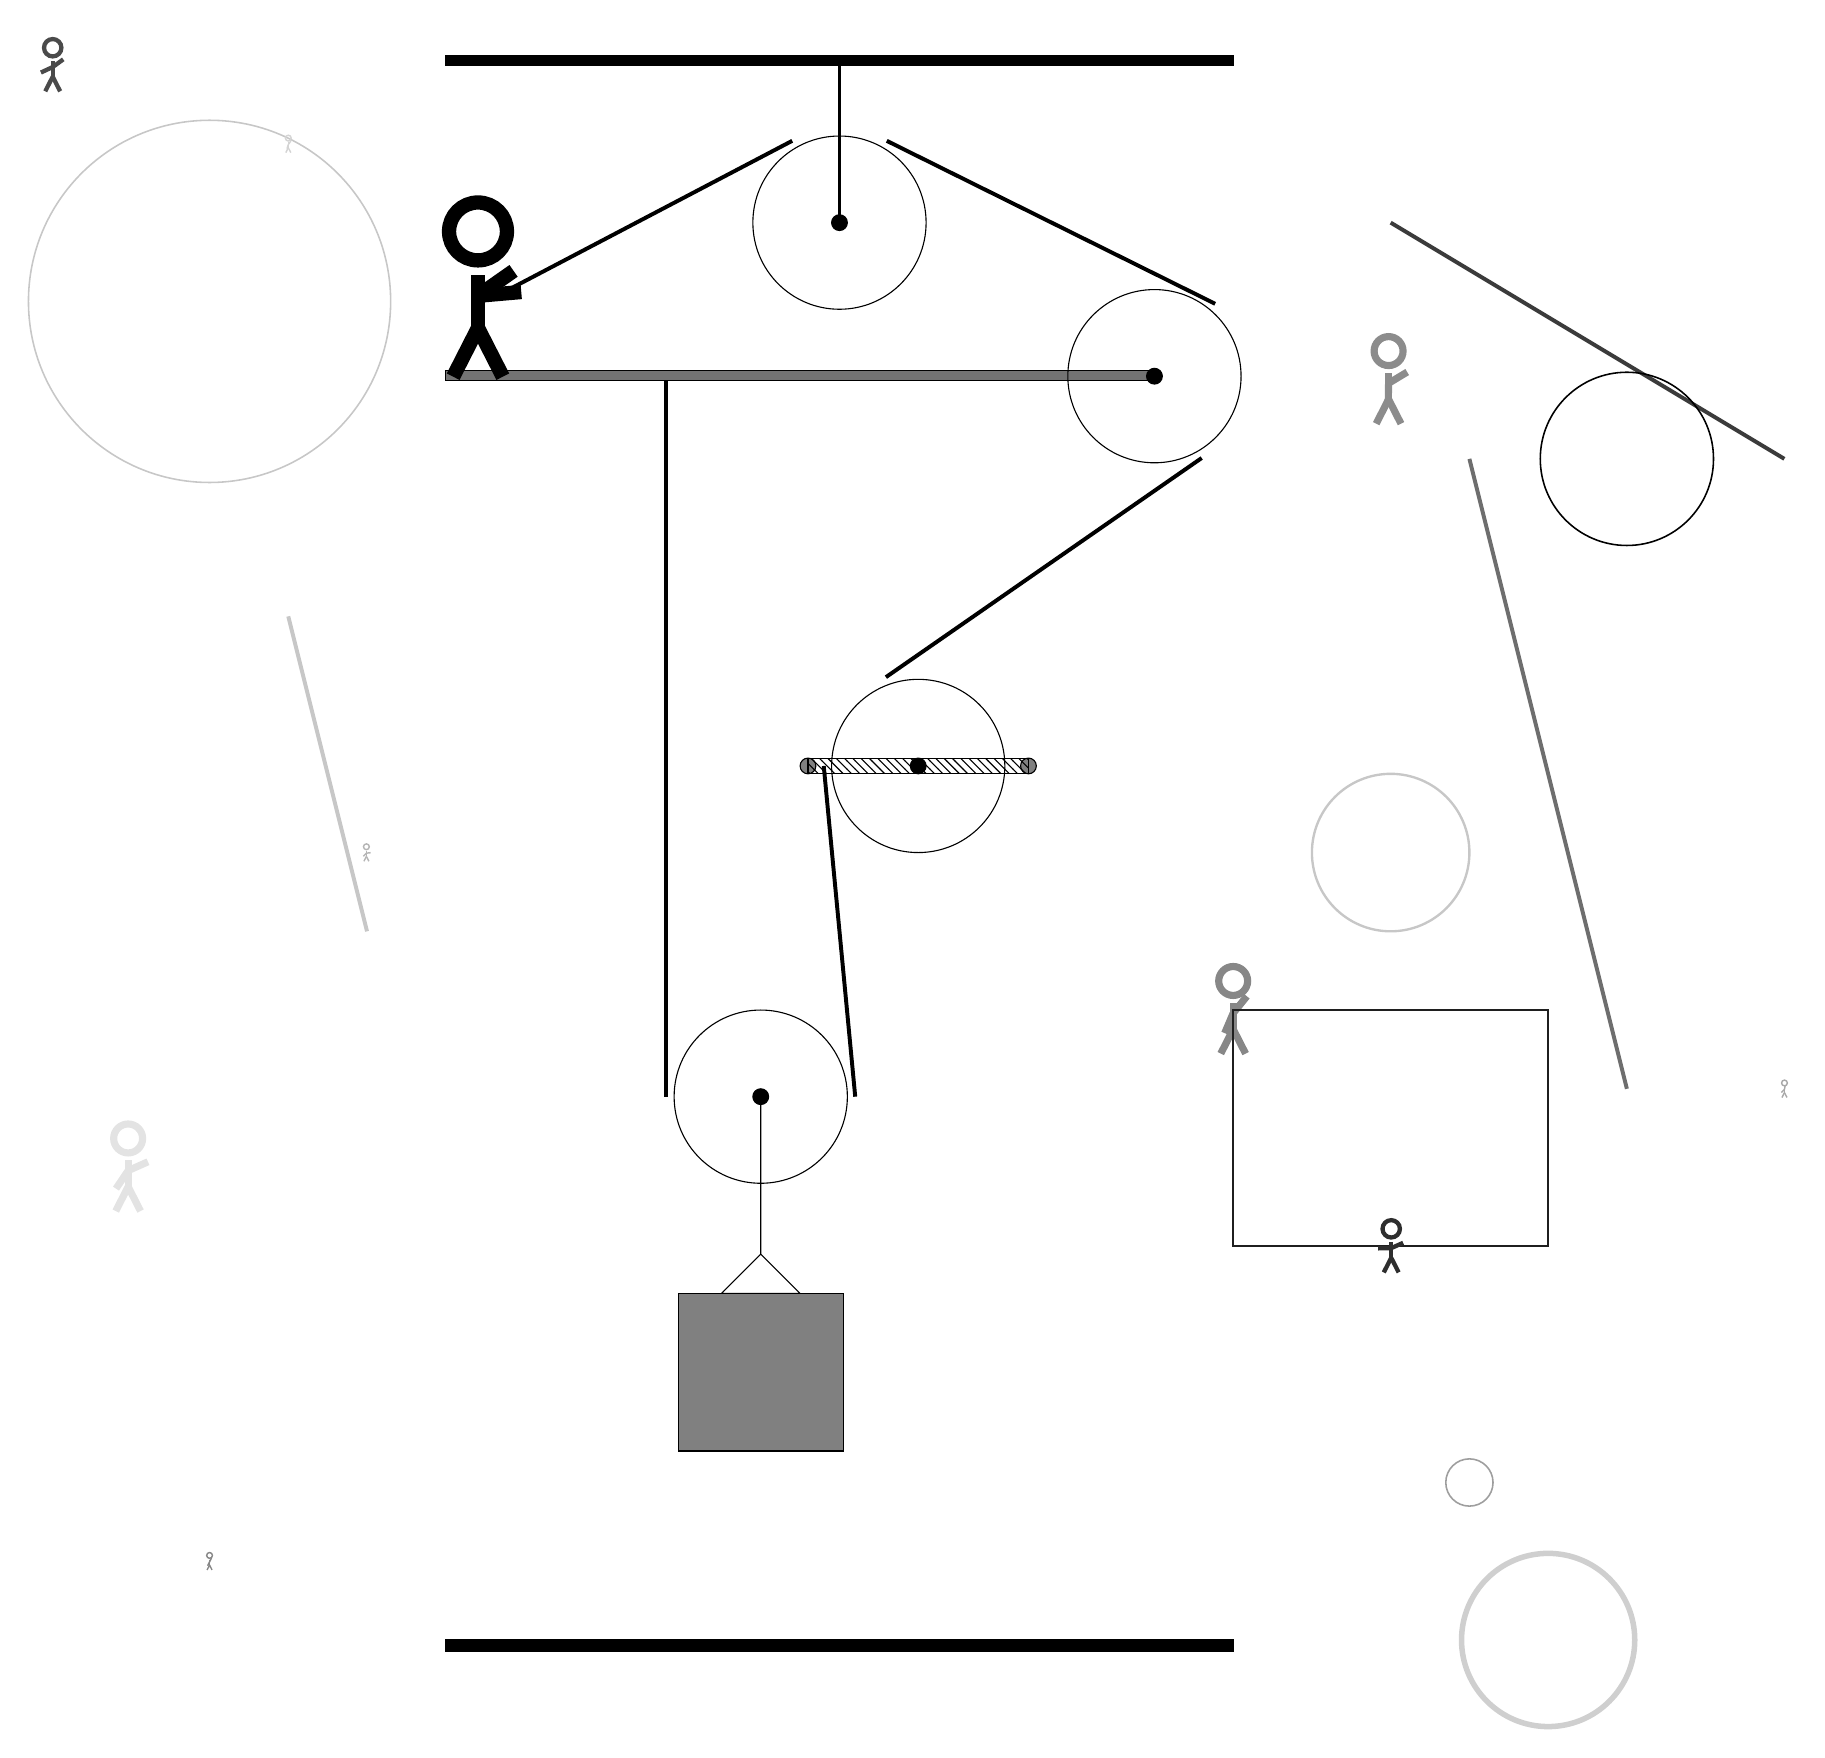
\begin{tikzpicture}
			%%%%% START %%%%%
			
			\draw[fill=black] (-2, 18) rectangle (8, 18.125);
			
			\draw[fill=black!55] (-2, 14) rectangle (7, 14.125);
			
			\draw (2, 4.9) circle (1.1);
			\draw[fill=black] (2, 4.9) circle (0.1);
			
			\draw (7, 14.05) circle (1.1);
			\draw[fill=black] (7, 14.05) circle (0.1);
			
			\draw[fill=white](4, 9.1) circle (1.1);
			\draw[fill=black] (4, 9.1) circle (0.1);
			\draw[fill=black!50] (2.6, 9.1) circle (0.1);
			\draw[fill=black!50] (5.4, 9.1) circle (0.1);
			\draw[pattern=north west lines, pattern color=black] (2.6, 9.2) rectangle (5.4, 9.0);
			
			\draw (3, 16) circle (1.1);
			\draw[fill=black] (3, 16) circle (0.1);
			\draw[line width=0.5mm] (3, 16) -- (3, 18);
			
			\draw (2, 4.9) -- (2, 2.9) -- (1.5, 2.4) -- (2.5, 2.4) -- (2, 2.9);
			\draw[fill=black!50] (0.95, 2.4) rectangle (3.05, 0.4);
			
			\draw[line width=0.5mm] (0.8, 14) -- (0.8, 4.9);
			\centerarc[line width=0.5mm](2, 4.9)(180:360:1.2000000000000002);
			\draw[line width=0.5mm](3.2, 4.9) -- (2.8, 9.1);
			\centerarc[line width=0.5mm](4, 9.1)(110:180:1.2000000000000002);
			\draw[line width=0.5mm](3.5896, 10.2276) -- (7.6, 13.0108);
			\centerarc[line width=0.5mm](7, 14.05)(-60:50:1.2000000000000002);
			\draw[line width=0.5mm](7.7714, 14.9692) -- (3.6, 17.0392);
			\centerarc[line width=0.5mm](3, 16)(60:120:1.2000000000000002);
			\draw[line width=0.5mm](2.4, 17.0392) -- (-1.2, 15.15);
			
			\node at (-1.5, 15.15) {\Strichmaxerl[10][-175][35]};
			
			\draw [line width=0.2mm, color=black!22](-5, 15) circle (2.3);
			
			\draw [line width=0.7mm, color=black!19](12, -2) circle (1.1);
			\draw [line width=0.2mm, color=black!38](11, 0) circle (0.3);
			\draw[line width=0.5mm, color=black!77](10, 16) -- (15, 13);
			\draw[line width=0.5mm, color=black!57](13, 5) -- (11, 13);
			\node[line width=0.7mm, color=black!29] at (-3, 8) {\Strichmaxerl[1][46][7]};
			\node[line width=0.2mm, color=black!11] at (-6, 4) {\Strichmaxerl[5][56][24]};
			\node[line width=0.5mm, color=black!47] at (-5, -1) {\Strichmaxerl[1][64][64]};
			\node[line width=0.7mm, color=black!71] at (-7, 18) {\Strichmaxerl[3][25][36]};
			
			\node[line width=0.4mm, color=black!47] at (8, 6) {\Strichmaxerl[5][67][51]};
			\node[line width=0.2mm, color=black!45] at (10, 14) {\Strichmaxerl[5][89][31]};
			
			\draw[line width=0.3mm, color=black!88] (8, 3) rectangle (12, 6);
			\node[line width=0.6mm, color=black!82] at (10, 3) {\Strichmaxerl[3][1][24]};
			\node[line width=0.5mm, color=black!17] at (-4, 17) {\Strichmaxerl[1][72][54]};
			\draw [line width=0.2mm, color=black!100](13, 13) circle (1.1);
			\draw[line width=0.5mm, color=black!22](-3, 7) -- (-4, 11);
			
			\draw [line width=0.3mm, color=black!22](10, 8) circle (1.0);
			\node[line width=0.2mm, color=black!34] at (15, 5) {\Strichmaxerl[1][44][80]};
			
			\draw[fill=black] (-2, -2) rectangle (8, -2.15);
			
			%%%%% END %%%%%
		\end{tikzpicture}
	\end{figure}	
\end{document}